\let\negmedspace\undefined
\let\negthickspace\undefined
\documentclass[journal]{IEEEtran}
\usepackage[a5paper, margin=10mm, onecolumn]{geometry}
%\usepackage{lmodern} % Ensure lmodern is loaded for pdflatex
\usepackage{tfrupee} % Include tfrupee package

\setlength{\headheight}{1cm} % Set the height of the header box
\setlength{\headsep}{0mm}     % Set the distance between the header box and the top of the text

\usepackage{gvv-book}
%\usepackage{gvv}
\usepackage{cite}
\usepackage{amsmath,amssymb,amsfonts,amsthm}
\usepackage{algorithmic}
\usepackage{graphicx}
\usepackage{textcomp}
\usepackage{xcolor}
\usepackage{txfonts}
\usepackage{listings}
\usepackage{enumitem}
\usepackage{mathtools}
\usepackage{gensymb}
\usepackage{comment}
\usepackage[breaklinks=true]{hyperref}
\usepackage{tkz-euclide} 
\usepackage{listings}
\usepackage{gvv}                                        
\def\inputGnumericTable{}                                 
\usepackage[latin1]{inputenc}                                
\usepackage{color}                                            
\usepackage{array}                                            
\usepackage{longtable}                                       
\usepackage{calc}                                             
\usepackage{multirow}                                         
\usepackage{hhline}                                           
\usepackage{ifthen}                                           
\usepackage{lscape}
\begin{document}

\bibliographystyle{IEEEtran}

\title{2.4.13}
\author{EE25BTECH11019 - Darji Vivek M.}
{\let\newpage\relax\maketitle}

\renewcommand{\thefigure}{\theenumi}
\renewcommand{\thetable}{\theenumi}
\setlength{\intextsep}{10pt}
\numberwithin{figure}{enumi}
\renewcommand{\thetable}{\theenumi}

\textbf{Question}:\\
$\vec{B}-\vec{A}=3\vec{i}-\vec{j}+\vec{k}$ and $\vec{D}-\vec{C}=-3\vec{i}+2\vec{j}+4\vec{k}$ are two vectors.  
The position vectors of the points $\vec{A}$ and $\vec{C}$ are $6\vec{i}+7\vec{j}+4\vec{k}$ and $-9\vec{j}+2\vec{k}$, respectively.  
Find the position vectors of a point $\vec{P}$ on the line $\vec{A}\vec{B}$ and a point $\vec{Q}$ on the line $\vec{C}\vec{D}$ such that $\vec{Q}-\vec{P}$ is perpendicular to both $\vec{B}-\vec{A}$ and $\vec{D}-\vec{C}$.\\[4pt]
\hfill $\brak{10,2021}$

\solution \\[-2mm]

\begin{table}[h!]
\centering
\begin{tabular}{|c|c|}
\hline
Symbol & Meaning \\ \hline
$\vec{a}$ & $\myvec{6\\7\\4}$ (position vector of $\vec{A}$) \\ \hline
$\vec{c}$ & $\myvec{0\\-9\\2}$ (position vector of $\vec{C}$) \\ \hline
$\vec{d}_1$ & $\myvec{3\\-1\\1}$ (direction of $\vec{B}-\vec{A}$) \\ \hline
$\vec{d}_2$ & $\myvec{-3\\2\\4}$ (direction of $\vec{D}-\vec{C}$) \\ \hline
$\lambda,\mu$ & Parameters for $\vec{P},\vec{Q}$ on $\vec{A}\vec{B},\vec{C}\vec{D}$ respectively \\ \hline
\end{tabular}
\caption{Variables Used}
\label{tab:198-vars}
\end{table}

\textbf{Matrix Method:}\\
Points on the lines can be written as
\begin{align}
\vec{P}=\vec{a}+\lambda\vec{d}_1,\qquad
\vec{Q}=\vec{c}+\mu\vec{d}_2.
\end{align}
Then
\begin{align}
\vec{Q}-\vec{P}
=(\vec{c}-\vec{a})+\mu\vec{d}_2-\lambda\vec{d}_1.
\end{align}
Perpendicularity to both $\vec{d}_1$ and $\vec{d}_2$ gives
\begin{align}
\vec{d}_1^{\top}(\vec{Q}-\vec{P})=0,\qquad
\vec{d}_2^{\top}(\vec{Q}-\vec{P})=0.
\end{align}
This yields the $2\times 2$ linear system
\begin{align}
\underbrace{\myvec{\vec{d}_1^{\top}\vec{d}_1 & \vec{d}_1^{\top}\vec{d}_2\\[2pt]
\vec{d}_2^{\top}\vec{d}_1 & \vec{d}_2^{\top}\vec{d}_2}}_{\text{Gram matrix }G}
\myvec{\lambda\\ \mu}
=
-\myvec{\vec{d}_1^{\top}(\vec{c}-\vec{a})\\[2pt]
\vec{d}_2^{\top}(\vec{c}-\vec{a})}.
\label{eq:gram}
\end{align}

Compute the required dot products:
\begin{align}
\vec{d}_1=\myvec{3\\-1\\1},\quad
\vec{d}_2=\myvec{-3\\2\\4},\quad
\vec{c}-\vec{a}=\myvec{-6\\-16\\-2}.
\end{align}
\[
\vec{d}_1^{\top}\vec{d}_1=11,\quad
\vec{d}_2^{\top}\vec{d}_2=29,\quad
\vec{d}_1^{\top}\vec{d}_2=\vec{d}_2^{\top}\vec{d}_1=-7,
\]
\[
\vec{d}_1^{\top}(\vec{c}-\vec{a})=-4,\qquad
\vec{d}_2^{\top}(\vec{c}-\vec{a})=-22.
\]
Hence, from \eqref{eq:gram},
\begin{align}
\myvec{11 & -7\\ -7 & 29}\myvec{\lambda\\ \mu}=\myvec{4\\ 22}.
\end{align}
Solving,
\begin{align}
\lambda=-1,\qquad \mu=1.
\end{align}

Therefore,
\begin{align}
\vec{P}&=\vec{a}+\lambda\vec{d}_1
=\myvec{6\\7\\4}-\myvec{3\\-1\\1}
=\boxed{\myvec{3\\8\\3}},\\[4pt]
\vec{Q}&=\vec{c}+\mu\vec{d}_2
=\myvec{0\\-9\\2}+\myvec{-3\\2\\4}
=\boxed{\myvec{-3\\-7\\6}}.
\end{align}

\textbf{Verification:}
\begin{align}
\vec{Q}-\vec{P}=\myvec{-6\\-15\\3},\quad
\vec{d}_1^{\top}(\vec{Q}-\vec{P})=0,\quad
\vec{d}_2^{\top}(\vec{Q}-\vec{P})=0,
\end{align}
confirming $\vec{Q}-\vec{P}\perp \vec{B}-\vec{A}$ and $\vec{Q}-\vec{P}\perp \vec{D}-\vec{C}$.

\begin{figure}[H]
\centering
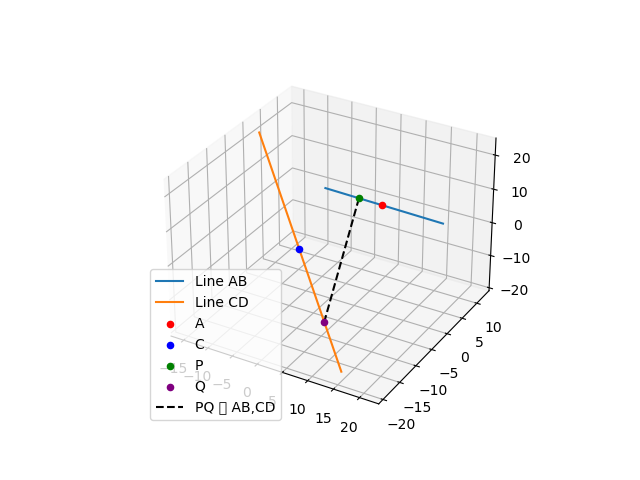
\includegraphics[width=0.75\columnwidth]{figs/3.png}
\caption{\centering plot}
\label{fig:placeholder_125}
\end{figure}

\end{document}
